\documentclass[11pt,a4paper,titlepage, ngerman]{article}

\usepackage[utf8]{inputenc}	% Diese Pakete sind
\usepackage[T1]{fontenc}		% für die Verwendung 
\usepackage{ngerman}			% von Umlauten im tex-file
\usepackage{lmodern}			% Schriftart, die am Bildschirm besser lesbar ist
\usepackage{graphicx}			% Zum Einbinden von Formeln
\usepackage{url}					% Zur Darstellung von Webadressen
\usepackage{siunitx}
\usepackage{amsmath}			% für equation*
\usepackage{subcaption}

\begin{document}	
	\begin{titlepage}
		\centering
			{\scshape\LARGE Versuchsbericht zu \par}
		\vspace{1cm}
			{\scshape\huge S1 -- Was ist Experimentieren?\par}
		\vspace{2.5cm}
			{\LARGE Gruppe 10 Mi\par}
		\vspace{0.5cm}
			{\large Alex Oster (E-Mail: a\_oste16@uni--muenster.de) \par}
			{\large Jonathan Sigrist (E-Mail: j\_sigr01@uni--muenster.de ) \par}
		\vfill
			durchgeführt am 18.10.2017\par
			betreut von\par
			{\large Dr. Anke \textsc{Schmidt}}		
		\vfill		
			{\large \today\par}
	\end{titlepage}	
	
	\tableofcontents	
	\newpage
		
	\section{Einleitung}
		\label{Einleitung}		
		In diesem Bericht, zur ersten experimentellen Übung, beschäftigen wir uns mit der Frage, was genau man unter dem Begriff \glqq Experimentieren\grqq\ verstehen sollte. Dazu betrachten wir zunächst folgende Fragen:	
		\begin{enumerate}			
			\item Was ist mit \glqq Messgröße\grqq\ gemeint?
			\item Warum führt man Experimente in der Naturwissenschaft durch? und
			\item Weshalb kann der \glqq wahre Wert\grqq\ einer Messgröße niemals bestimmt werden?			
		\end{enumerate}			
			Zur Beantwortung dieser Fragen, wenden wir uns nun drei einfachen Versuchen zu, welche die Bedeutung von Messungenauigkeiten durch unterschiedliche Messverfahren verdeutlichen sollen. 
			
			In dem ersten Versuch haben wir die Leerlaufspannung einer 9V-Batterie gemessen, in dem zweiten Versuch die Länge eines \glqq STABILO point 88\grqq\ Stiftes und in dem dritten Versuch dann die Zeit, die Kugeln verschiedener Masse zum Herunterrollen einer schiefen Ebene benötigen.
						
			Die Auswertungen dieser Versuche werden wir abschließend verwenden, um die oben gestellten Fragen zu beantworten und um damit den Begriff \glqq Experimentieren\grqq {} zu erklären.
	
	\newpage		
	\section{Durchführung}
		\label{Durchführung}
				
		\subsection{Versuch 1: Leerlaufspannung}
			\label{2.1}		
			In diesem Versuch geht es um die Messung der Leerlaufspannung einer \SI{9}{\V}-Batterie mit Hilfe eines digitalen Multimeters. 
			
			Wir fragen uns zunächst, welche Werte für die Leerlaufspannung $U_0$ realistisch wirken und stellen eine Hypothese bzw. einen Erwartungsbereich auf.
					
			\subsubsection{Vorwissen und Aufstellen einer Hypothese}
				\label{2.1.1}			
				Da es sich um eine \SI{9}{\V}-Batterie handelt und keine negativen Werte für $U_0$ vorliegen können, schließen wir darauf, dass der Wert für die Leerlaufspannung sich mindestens im Bereich von \SIrange{0}{9}{\V} befinden sollte.
				
				Das, am Boden der Batterie, gegebene Mindesthaltbarkeitsdatum (\glqq 2020\grqq) wurde noch nicht überschritten, weswegen bis dahin die \SI{9}{\V} garantiert sein sollten. Also folgern wir, dass die Batterie, im unbenutzten Falle, auch mehr als \SI{9}{\V} Leerlaufspannung besitzen könnte.
				
				Deswegen haben wir unseren Erwartungsbereich von \SIrange{0}{9}{\V} auf \SIrange{0}{10}{\V} erweitert, wie in Abb. \ref{fig:spannung} zu sehen ist.			
				\begin{figure}
					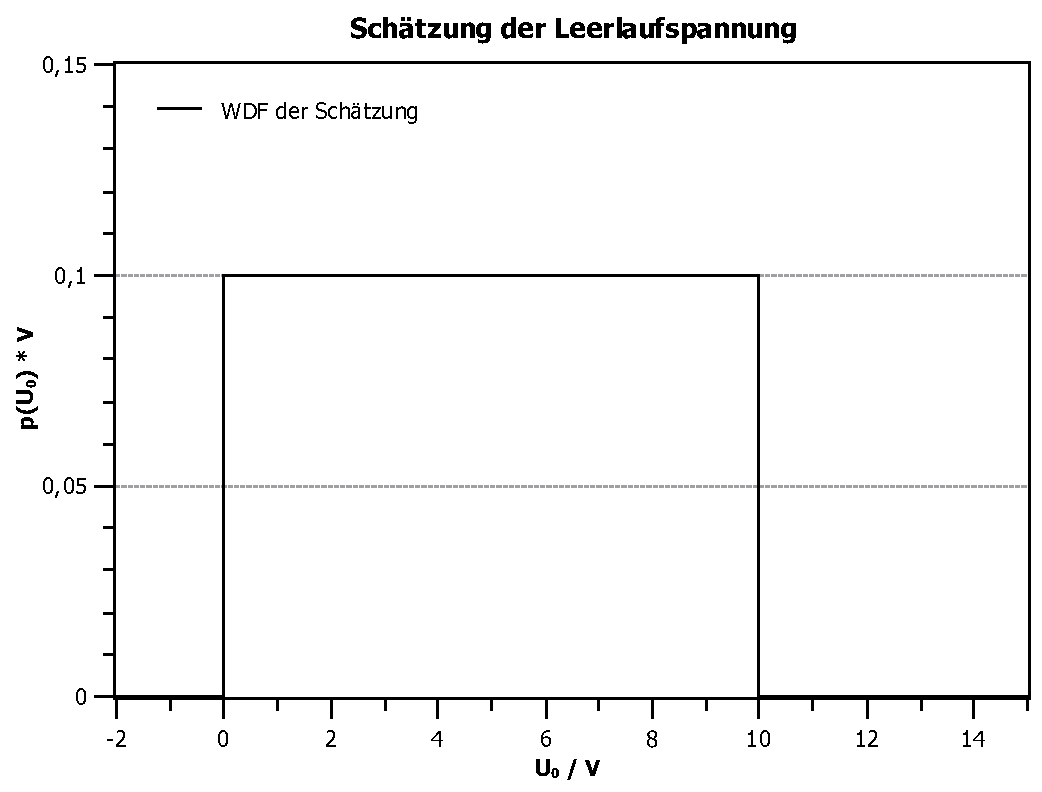
\includegraphics[width=\textwidth]{Spannungsschaetzung_2.pdf}
					\caption{Schätzung der Leerlaufspannung.}
					\label{fig:spannung}
				\end{figure}		
				\begin{figure}
					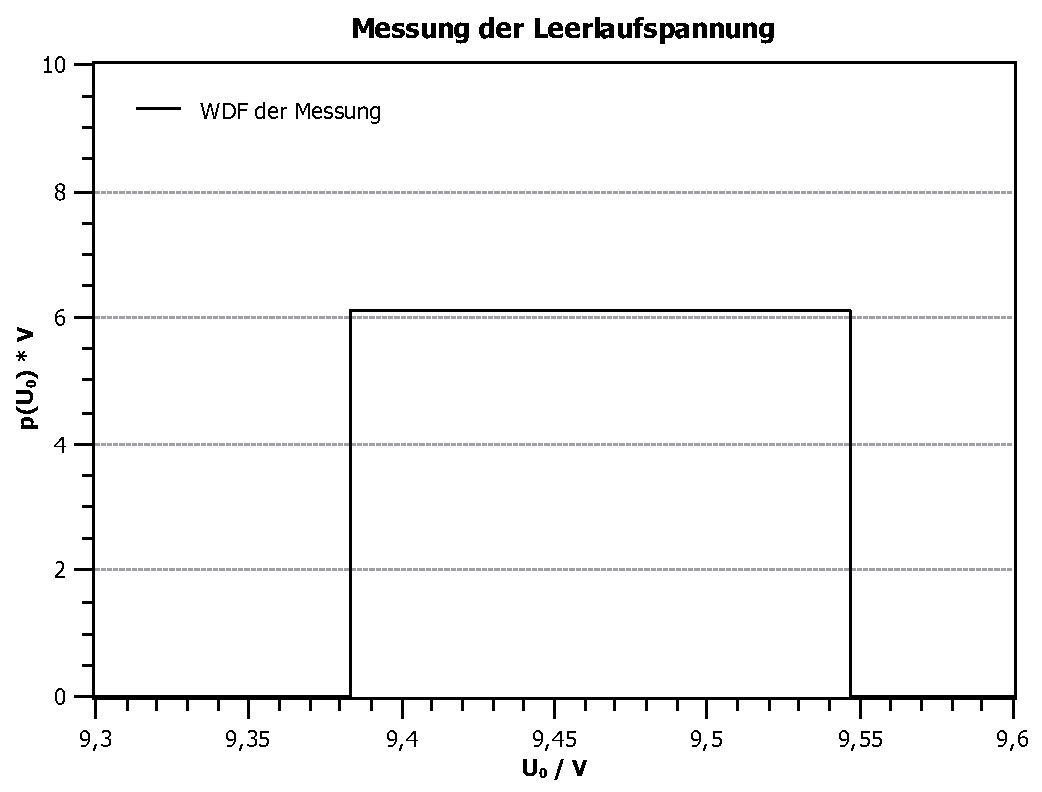
\includegraphics[width=\textwidth]{Spannungsmessung_2.pdf}
					\caption{Messung der Leerlaufspannung.}
					\label{fig:spannung2}
				\end{figure}	
				
			\subsubsection{Messwerte, Ungenauigkeitsbetrachtung und Ergebnis}
				\label{2.1.2}	
					
				Zur Durchführung der Messung haben wir das Multimeter erst auf den zu erwartenden Messbereich von ungefähr \SI{10}{\V} kalibriert und dann mit einfachen Kabeln an die \SI{9}{\V}-Batterie angeschlossen.
						
				Die, von dem Gerät, gemessenen Werte schwankten zwischen \SI{9,46}{\V} und \SI{9,47}{\V}, der Idealwert ist somit \SI{9,465}{\V}. Da das Messgerät jedoch rundet, betrachten wir eigentlich Werte im Bereich von \SIrange{9,455}{9,475}{\V}. Mit $u_1 =  \frac{a}{2\sqrt{3} }$ und $a=0,02$ (Abstand der Intervall Grenzen) ergibt sich eine Unsicherheit von $u_1 = \SI{0,0058}{\V}$.
				Zudem besitzt das Messgerät eine Ungenauigkeit von $0.5\%$ des angegebenen Wertes, also einer weiteren Unsicherheit von  $u_2 = \SI{0,047}{\V}$. 
				 	
				Aus den beiden Unsicherheiten $u_1=\SI{0,0058}{V}$ und $u_2= \SI{0,047}{\V}$ berechnet sich die kombinierte Unsicherheit $u$ mit
				\begin{equation*}
					u = \sqrt{\left( u_1 \right)^2 + \left( u_2 \right)^2}
					= \sqrt{\left( \SI{0,0058}{V} \right)^2 + \left( \SI{0,047}{\V} \right)^2}
					= \SI{0,0474}{\V}
				\end{equation*}
				weswegen der eigentliche Wert, wie Abb. \ref{fig:spannung2} dargestellt, bei \SI{9,465 \pm 0,0474}{\V}  liegt.
			
			\subsubsection{Schlussfolgerung}
				
				Wie erwartet, liegt der gemessene Wert zwischen \SI{0}{\V} und \SI{10}{\V}. Darüber hinaus sogar zwischen \SI{9}{\V} und \SI{10}{\V}. Wir können also davon ausgehen, dass die Batterie weitgehend unbenutzt ist und somit für weitere Reihen an Experimenten einen Nutzen finden kann.
									
		\subsection{Versuch 2: Längenmessung}
			\label{2.2}	
			
			Der zweite Versuch beschäftigt sich mit der Messung der Länge eines Stiftes. Und auch hier fragen wir uns zuerst, welche Werte für die Länge des Stiftes in Frage kommen.
			
			\subsubsection{Schätzung}
				\label{2.2.1}	
				
				Die Stiftlänge haben wir über die Spannbreite von Daumen und Zeigefinger in ein Intervall von \SIrange{15}{20}{\cm} abgeschätzt. Dies haben wir in Abb. \ref{fig:laenge} dargestellt.
				
				\begin{figure}
					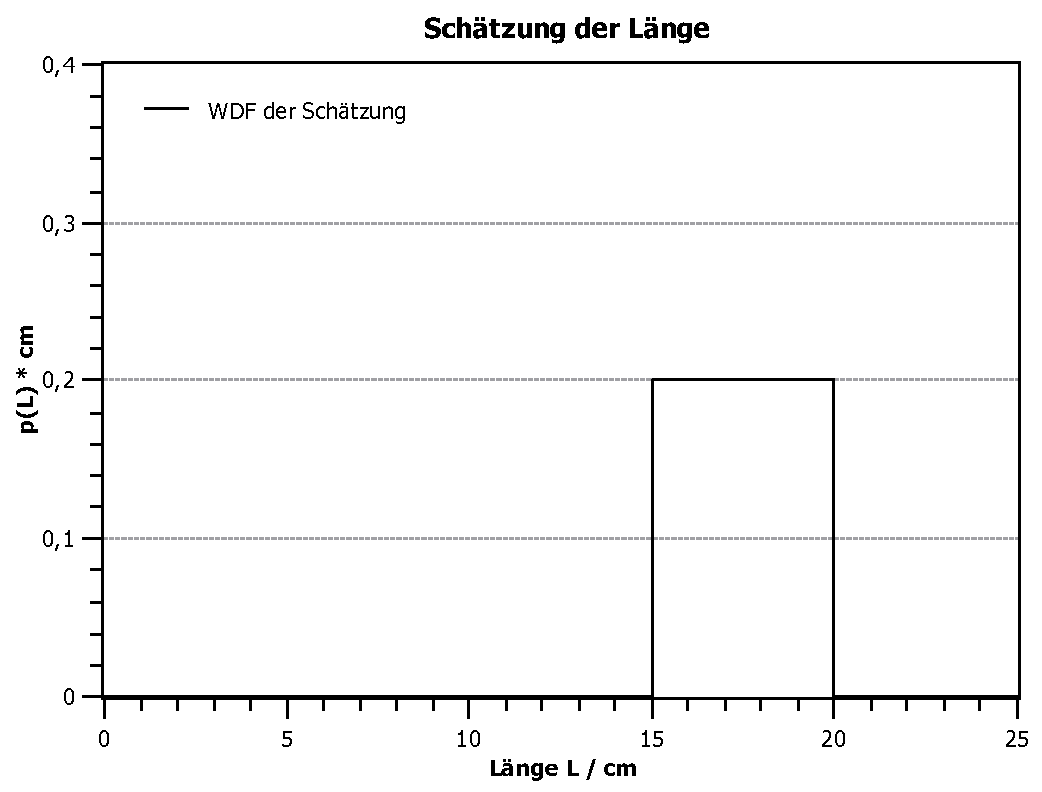
\includegraphics[width=\textwidth]{Laengenschaetzung_2.pdf}				
					\caption{Schätzung der Stiftlänge.}
					\label{fig:laenge}
				\end{figure}
				\begin{figure}
					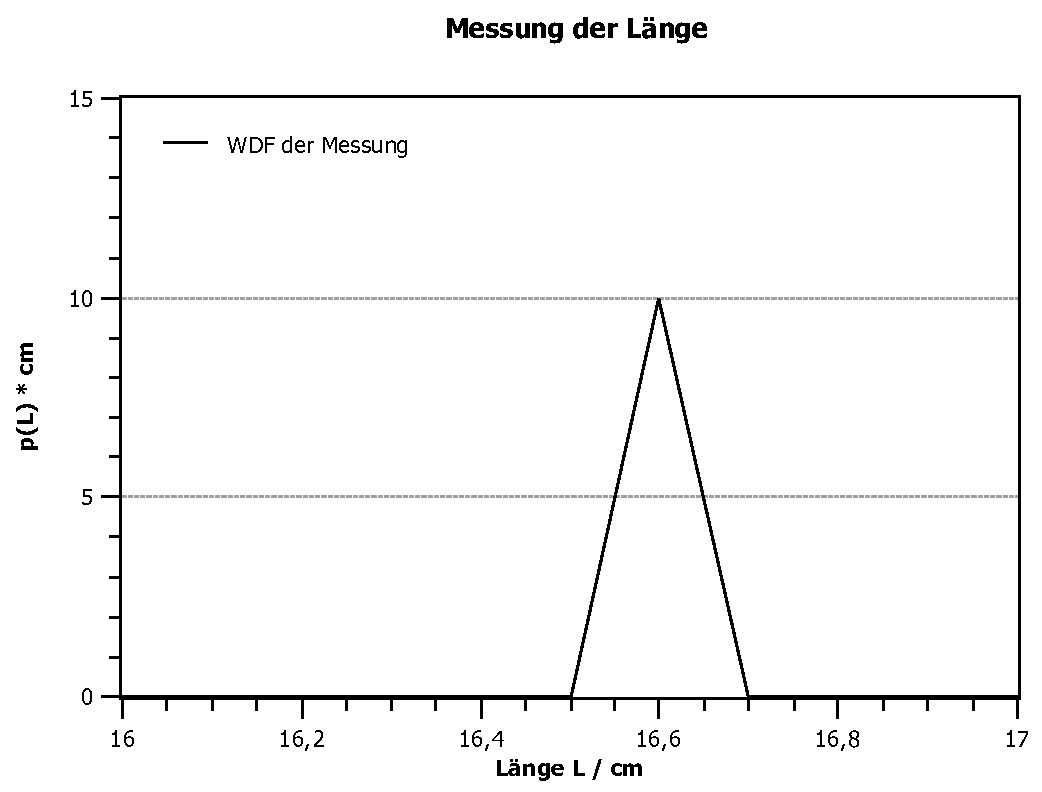
\includegraphics[width=\textwidth]{Laengenmessung_2.pdf}				
					\caption{Messung der Stiftlänge.}
					\label{fig:laenge2}
				\end{figure}
			
			\subsubsection{Messung}
				\label{2.2.2}
				
				Mit Hilfe eines handelsüblichen Maßbandes haben wir die Messung der Stiftlänge durchgeführt. 
				Sie ergab eine Länge von ca. \SI{16,6}{\cm} von beiden Seiten. Dieser Messung teilten wir einen Toleranzbereich von maximal \SI{0,1}{\cm} zu (vgl. Abb. \ref{fig:laenge2}), da für die Unsicherheit des Maßbandes kein realistischer Wert\footnote{eine Ungenauigkeit von \SI{6}{\cm} auf \SI{2}{\m} war gegeben} gegeben war.
			
			\subsubsection{Schlussfolgerung}
				
				Mit der Standardunsicherheit für Dreiecksverteilungen, ergibt sich 
				\begin{equation*}
					u = \frac{a}{2 \sqrt{6}} = \frac{\SI{0,2}{\cm}}{2 \sqrt{6}} = \SI{0,041}{\cm}
				\end{equation*}
				ein Wert von \SI{16,6 \pm 0,041}{\cm} für die Länge des Stiftes. Dieser Wert liegt in unserem geschätzten Bereich und bestätigt somit unsere Annahme.
		\subsection{Versuch 3: Schiefe Ebene}
			\label{2.3}	
			
			In dem dritten Versuch messen wir die Zeit, die zwei Kugeln aus verschiedenem Material für das Herunterrollen einer schiefen Ebene benötigen, um die Frage zu beantworten, welche der Kugeln schneller rollt und warum die andere Kugel langsamer rollt.		
				
			\subsubsection{Hypothese}
				\label{2.3.1}
					
				Wir vermuten, dass bei der Verwendung von einer Metall- und einer Holzkugel, die Metallkugel schneller die schiefe Ebene herunter rollt als die Kugel aus Holz, da die Holzkugel eine größere Rollreibung besitzt und leichte ist als die Metallkugel. 
				
			\subsubsection{Messung, Beobachtung und Messwerte}
				\label{2.3.2}
				
				Um die Hypothese zu verifizieren bzw. falsifizieren, haben wir eine Holz- und eine Metallkugel, mit gleichem Radius, mehrfach eine schiefe Ebene herunter rollen lassen und dabei die Zeit gemessen, die sie dafür gebraucht haben.
				
				Dabei haben wir kleine Ungenauigkeiten, welche u.A. durch den Luftwiderstand und Reibung aufgerufen werden, nicht genauer betrachtet. 
				
				Diese Messung haben wir 15 mal pro Kugel durchgeführt, sodass der Mittelwert über alle Messungen sich mit jeder neuen Messung nicht merklich geändert hat: \SI{1.713}{\s} für die Metallkugel und \SI{1.791}{\s} für die Holzkugel. Der Mittelwert $\mu$ berechnet sich wie folgt:
				\begin{equation*}
					 \sum\limits_{i=1}^n \frac{t_i}{n} = \bar{t}, \text{wobei $t_i$ die Zeit für die i-te Messung ist}
				\end{equation*}		
				
				\begin{figure}
					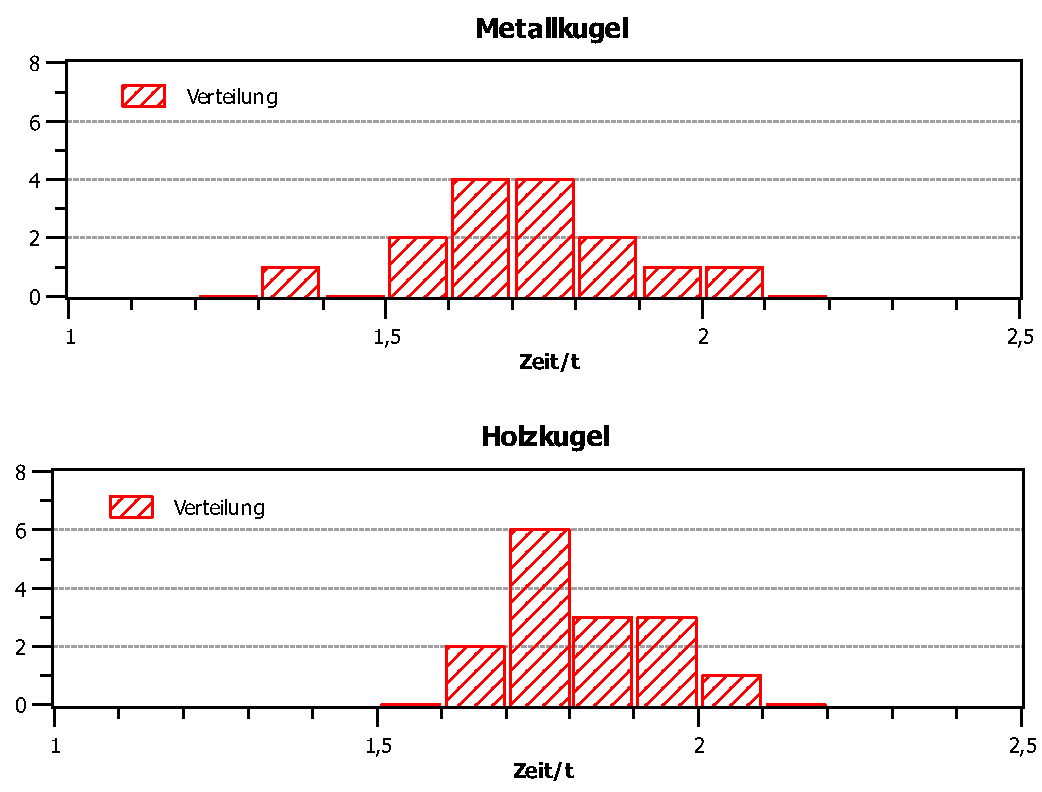
\includegraphics[width=\textwidth]{Histogramm_2.pdf}
					\caption{Verteilung der Messwerte.}
					\label{HistogrammV3}							
				\end{figure}
				\begin{figure}	
						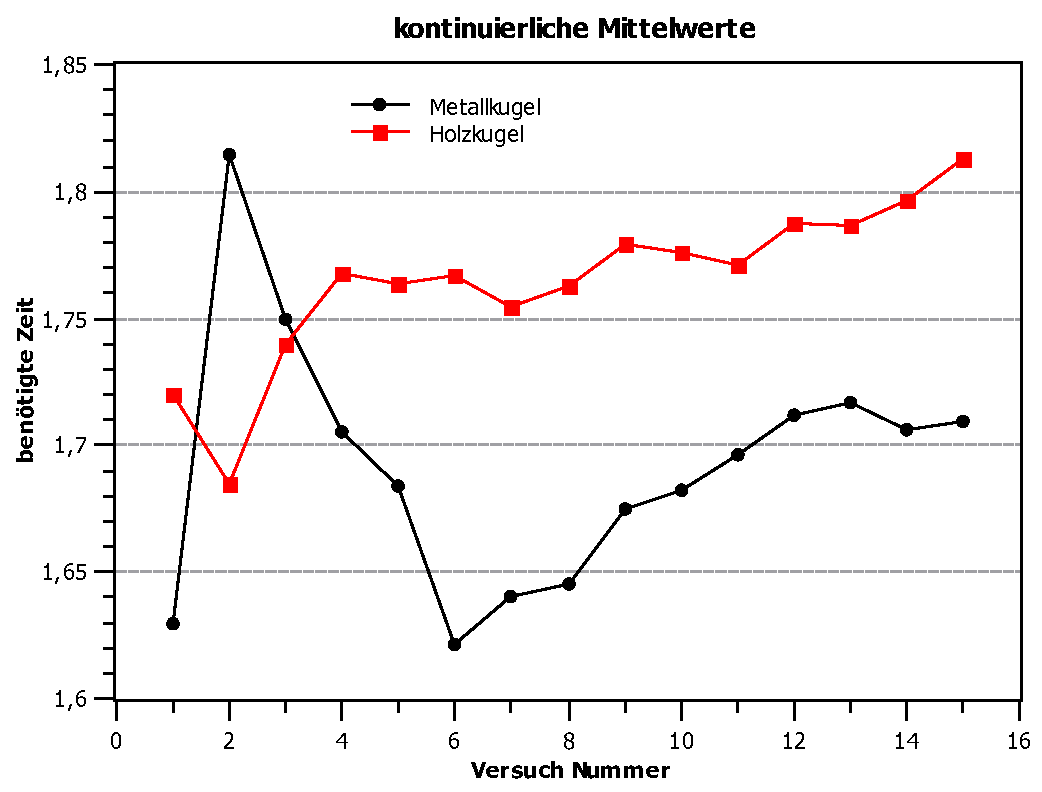
\includegraphics[width=\textwidth]{Mittelwerte_2.pdf}
						\caption{Entwicklung der Mittelwerte.}
						\label{MittelwerteV3}										
				\end{figure}								
				\begin{table}
					\label{Tab:VerteilungsWerte}
					\centering
					\begin{tabular}{l|SSS}
						\hline
						& {$\bar{t}$} & {$\sigma$} & {$u$} \\ \hline
						Metallkugel & 1,709 & 0,1512 & 0,039\\
						Holzkugel & 1,813 & 0,1035 & 0,0267\\ \hline
					\end{tabular}
					\caption{Mittelwert, Standardabweichung und Standardunsicherheit nach 15 Messungen.}
				\end{table}					
				Die Werte für Standardabweichungen und Mittelwerte nach 15 Messungen sind in Tab. 1 dargestellt, wobei sich Standardabweichung und -Unsicherheit wie folgt berechnen:
				
				\begin{equation*}
					\sigma = u(t_i) = \sqrt{\frac{1}{n-1} \sum_{i=1}^{n} (t_i - \bar{t})^2} \\			
				\end{equation*} 				
				für den Mittelwert:
				\begin{equation*}
					u(\bar{t}) = \frac{u(t_i)}{\sqrt{n}}
				\end{equation*}				
				Trotz 15 Messungen hat sich der Mittelwert für die Holzkugel noch um ca. \SI{0.02}{s} von dem vorherigen Mittelwert unterschieden. Das könnte an ungenauer Zeitmessung gelegen haben, weswegen weitere Messungen mit Sicherheit ein genaueres Ergebnis geliefert hätten.
				
				Außerdem haben wir zudem noch das zeitgleiche Herunterrollen beider Kugeln betrachtet und festgestellt, dass wenn die Holzkugel vorne ist, immer beide Kugeln gleichzeitig unten angekommen sind. War jedoch die Metallkugel vorne, so kam sie vor der Holzkugel unten an.	
			
			\subsubsection{Schlussfolgerung}
				\label{2.3.3}
				
				Der direkte Vergleich der Messwerte und die Beobachtung für zwei zeitgleich rollende Kugeln deuten darauf hin, dass die Hypothese, dass die Metallkugel schneller rollt, stimmt. 
				
				Da wir die Reibungseffekte nicht mit in die Messung einbringen konnten, erhalten wir, wenn wir diese ganz vernachlässigen, das Ergebnis, dass die Masse für die Geschwindigkeit verantwortlich ist, also schwerere Kugeln schneller rollen als Leichtere. 
				Sind die Reibungseffekte minimal, gilt dasselbe und wir können somit das Verhältnis von Masse und Geschwindigkeit bestätigen. 
				
	\newpage		
	\section{Beantwortung der Fragen}	
		\label{Diskussion}	
		
		Betrachten wir nun die Fragen aus \textbf{\ref{Einleitung} Einleitung}: 
		\begin{enumerate}
			\item \textit{Was ist mit \glqq Messgröße\grqq\ gemeint?} 
				\vspace{0.2cm}
				
				Eine Messgröße ist eine zu messende Größe bzw. das, was gemessen wird.
				Also ein Wert, der nicht genau bekannt ist und deshalb durch Messungen bestimmt werden soll.
				In \ref{2.1} war es die Leerlaufspannung $U_0$, in \ref{2.2} war es die Länge des Stiftes und in \ref{2.3} die Zeit, welche die Kugeln zum Herunterrollen benötigten.
				Messgrößen bieten uns die Möglichkeit, verschiedene Werte im selben Maß zu betrachten, um damit einzuordnen welche Werte größer, kleiner oder realistischer sind, wenn man sie mit dem Erwartungswert vergleicht. 			
			\item \textit{Warum führt man Experimente in der Naturwissenschaft durch?}
				\vspace{0.2cm}
				
				Das Ziel von Naturwissenschaften war es schon immer die Vorgänge der Natur zu erklären und Fragen zu beantworten. 
				Oft wurden und werden Experimente genutzt um Theorien und Hypothesen zu überprüfen. In unserem Falle, waren es Vermutungen, die wir durch kleine Versuche verifiziert haben.			
				Viele Sachverhalte werden jedoch erst durch in Experimenten gemachten Beobachtungen erkannt.
				Experimente tragen also auch aktiv an der Entdeckung von neuen Gesetzmäßigkeiten bei.	 
			\item \textit{Weshalb kann der \glqq wahre Wert\grqq\ einer Messgröße niemals bestimmt werden?}
				\vspace{0.2cm}
				
				Nein, der wahre Wert einer Messgröße kann nicht bestimmt werden. Unsere Versuche zeigen bereits, dass für die verschiedenen Messgrößen nur Erwartungswerte gefunden werden können, welche meistens ein \glqq breites Intervall\grqq\ aufgrund von Ungenauigkeiten beschreiben.
				Auch Seiteneffekte wie z. B. Reibung müssen für einen möglichst genauen Wert betrachtet werden, was das Finden eines \glqq wahren Werts\grqq\ durch Experimente zusätzlich erschwert.		
				Letztendlich kann ein Wert selbst bei sehr vielen Messungen aufgrund statistischer und systematischer Unsicherheiten nie auf einen \glqq wahren Wert\grqq\ reduziert werden.	
		\end{enumerate}
		Also was genau sollte man unter dem Begriff \glqq Experimentieren\grqq\ verstehen? 
		\glqq Experimentieren\grqq\ ist, wenn man unter kontrollierten Umgebungen eine Hypothese durch Messungen auf ihre Richtigkeit überprüft.	
		Hierbei ist das Ziel jedoch nicht die Bestimmung eines \glqq wahren Werts\grqq\, sondern der eines Erwartungswerts, da ein solcher sich in der Regel bestimmen lässt.
		Die Hypothese kann zum Beispiel vorherige Beobachtungen in einen größeren Zusammenhang stellen oder neue Gesetzmäßigkeiten voraussagen, die nun durch das Experiment belegt werden sollen.
		
\end{document} 